\chapter{Adaptive Mesh Refinement}\label{chapter:adaptive_mesh_refinement} 
% Something about move semantics
% No coarsening
% Adaptivity triggers
% Mortar here

Computers constantly increase in power, thanks to incremental progress made on known processes and
new architectures such as those described in Chapter~\ref{chapter:graphics_processing_units}.
However, processing power and memory are still limited and the size of problems studied has
increased in step with the available resources. It is still necessary to carefully manage those
limited resources in order to maximise the efficiency of simulations. Some flow regions may be more
interesting or harder to compute, benefiting from an increase in resolution. On the other hand, some
flow regions may have less happening in them or be easier to compute, and a decrease in resolution
may be acceptable.

\begin{figure}[H]
	\centering
	\subfloat[Mesh before refining]
	{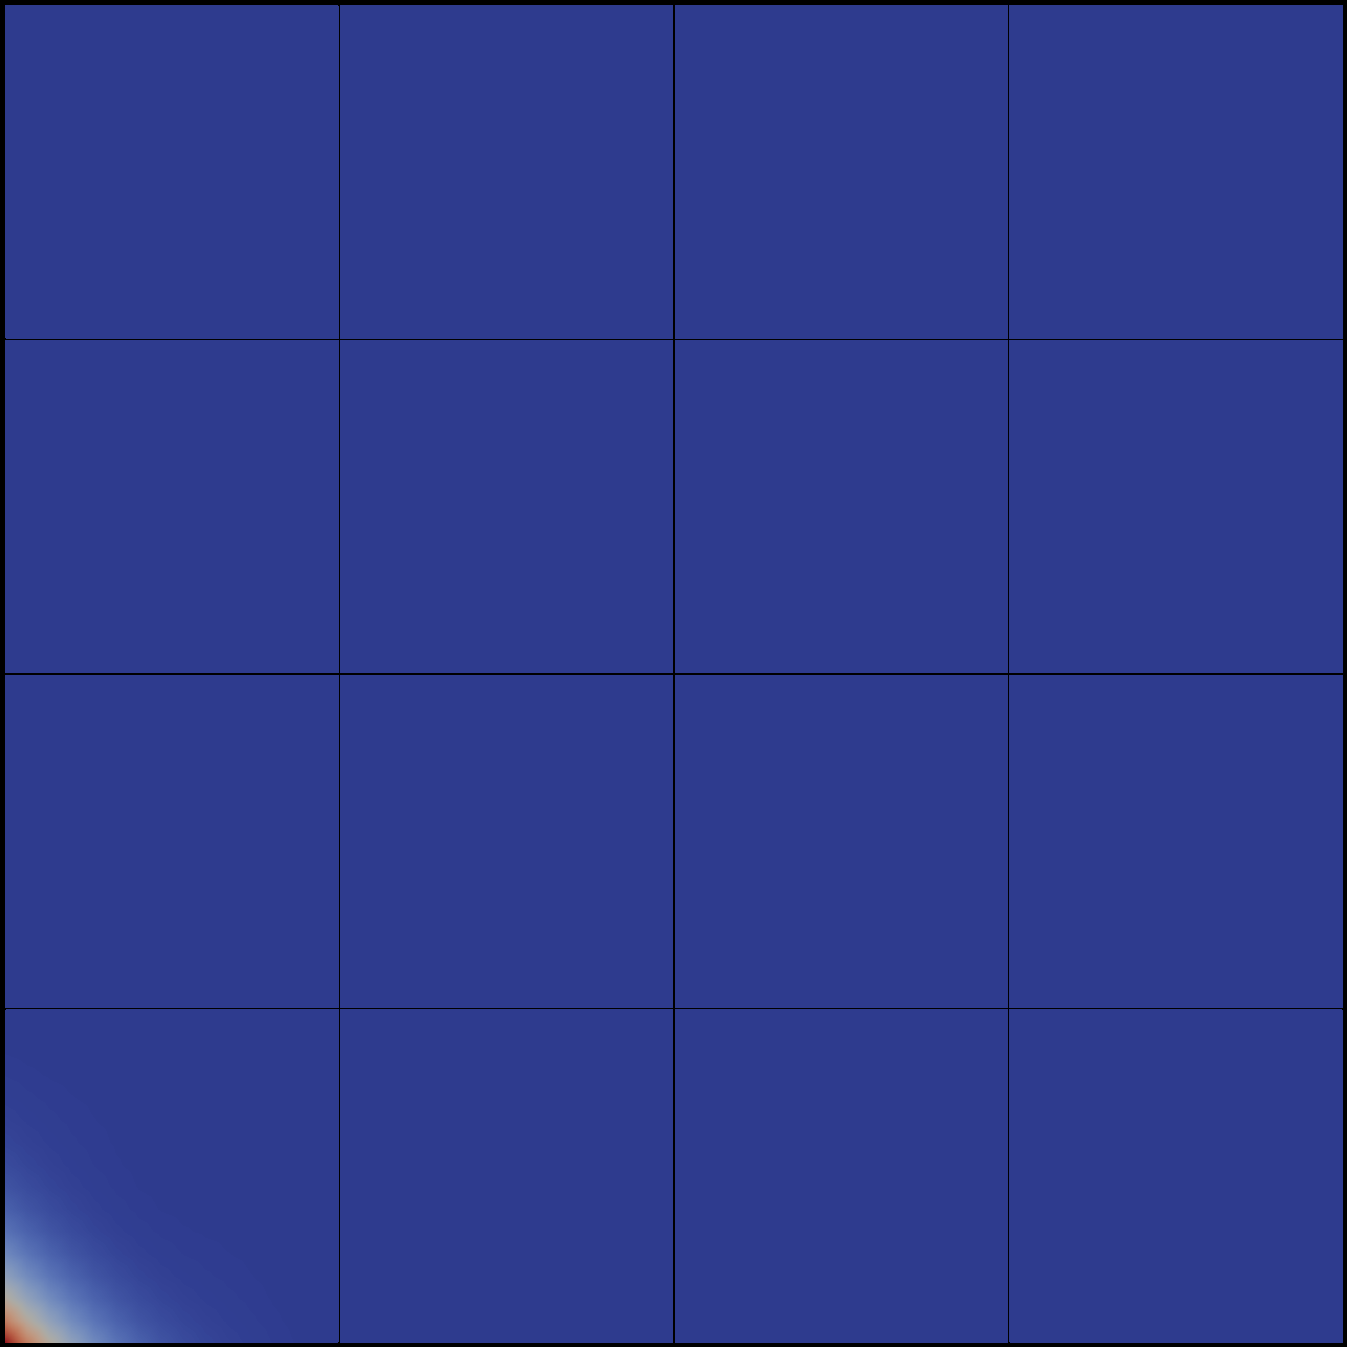
\includegraphics[width=0.45\textwidth]{Chapter_adaptive_mesh_refinement/media/mesh_initial}\label{fig:mesh_initial}}
	\hfill
	\subfloat[Mesh after refining]
	{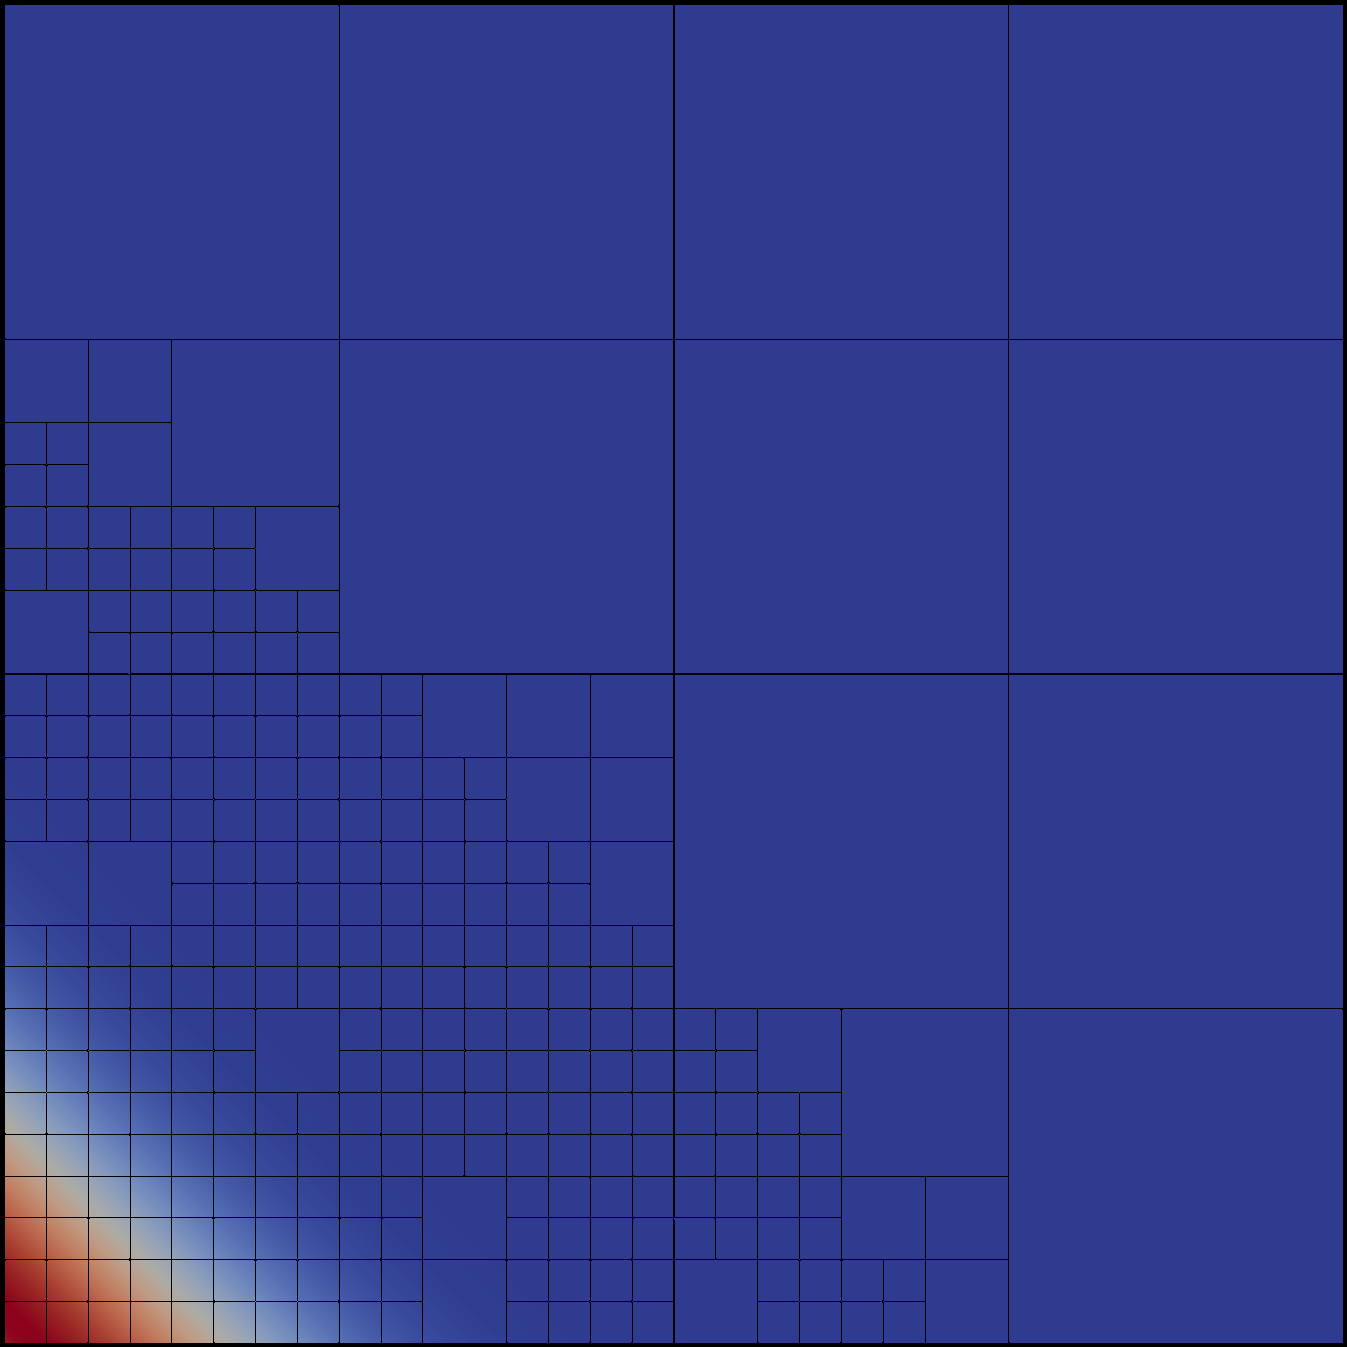
\includegraphics[width=0.45\textwidth]{Chapter_adaptive_mesh_refinement/media/mesh_refinement}\label{fig:mesh_after_refinement}}
	\caption{\Acrlong{acr:AMR}: The elements have split near the wave, where the solution is steeper. (a) Before refining (b) After refining}\label{fig:mesh_refinement}
\end{figure}

It is possible to increase the number of elements and/or the polynomial order of an entire mesh
before solving the problem. This increases resolution in important areas of the flow, but also
increases resolution everywhere else in the domain, where the increased computation cost provides no
benefit. It is sometimes possible to predict where to refine before solving the problem, such as
around static shock waves in predictable locations. In these cases, the mesh can be refined in those
areas before the computation starts. However, it is not always possible to know these areas
beforehand, or these areas may move as time advances if the problem is transient. The error may also
be higher in unforeseen areas.

\Acrlong{acr:AMR} is the process of altering the mesh as the computation goes, in areas where the
effect of that increase in resolution is most needed. To find out where to refine, the solution
error must be estimated, and a refinement method must be chosen. The error can be estimated by
extrapolating the value of the next mode in the spectral approximation, and the slope of the last
few modes can guide the choice of the refinement method. The two refinement methods studied here are
h-refinement and p-refinement, increasing the number of elements and the polynomial order,
respectively.

Once the mesh has been refined, the element boundaries can become geometrically or functionally
non-conforming. In order to accurately compute fluxes between the elements, we use the mortar element
method~\cite{Maday1989}. Mortar, in the form of faces, is added between the elements, and the
boundary solution is projected from the elements to the faces' own collocation points. After the
fluxes are computed on the faces, they are projected back from the faces to the elements. 

This whole process must be executed in parallel and with as much of the work as possible executed on
the \acrshort{acr:GPU}. \Acrshortpl{acr:GPU} are more efficient at working with fixed workloads
where all threads of a block execute the same instruction. Refining the mesh moves memory around and
can introduce additional branching if the elements have different polynomial orders or
non-conforming interfaces. The refinement process itself is also hard to implement on
\acrshortpl{acr:GPU}, as elements must either move, change their polynomial order or split into
multiple elements in parallel. If the different threads are not perfectly coordinated, risk the
chance of operating on the same destination memory location, creating race conditions.

When solving problems in parallel, the mesh will be split into blocks, each assigned to a process
and its \acrshort{acr:GPU}. As the mesh is refined, it is possible that the blocks are refined
unequally. This can lead to a load imbalance between the different \acrshortpl{acr:GPU}. As the
different \acrshortpl{acr:GPU} need to synchronise at each timestep, lightly-loaded
\acrshortpl{acr:GPU} will always be waiting for heavily-loaded \acrshortpl{acr:GPU}. The computation
time will therefore be driven by the most heavily-loaded \acrshort{acr:GPU}, and the speedup
incurred by parallelizing the program will be reduced. To improve this side effect of mesh
refinement, a dynamic load balancing algorithm will be implemented in
Chapter~\ref{chapter:load_balancing}.

\section{Strategies}\label{section:adaptive_mesh_refinement:refinement_strategies}

\subsection{p-refinement}\label{subsection:adaptive_mesh_refinement:refinement_strategies:p-refinement}

The first refinement strategy is p-refinement. When refining this way, elements increase their
polynomial order to increase their resolution. The lower-order solution is projected to the
higher-order collocation points. In this work, the polynomial order in increased in steps of 2, and
is required to be identical in the x and y directions. These restrictions are not necessary but are
implemented to simplify programming and increase GPU efficiency.

\begin{figure}[H]
	\centering
	\includesvg[width=0.6\textwidth]{Chapter_adaptive_mesh_refinement/media/p-adaptivity_N4_N6}
	\caption{2D p-refinement: The element's polynomial order is increased from 4 to 6, with 5 to 7 collocation points respectively.}\label{fig:p-refinement}
\end{figure}

\subsection{h-refinement}\label{subsection:adaptive_mesh_refinement:refinement_strategies:h-refinement}

The second refinement strategy is h-refinement\@. h-refinement splits single elements into several
elements occupying the same space. In this work we exclusively deal with quadrilaterals, and these
elements split into four smaller elements when h-refining for the same reasons as stated above. The
solution is projected from the initial big element to each of the four offspring elements.

\begin{figure}[H]
	\centering
	\includesvg[width=0.6\textwidth]{Chapter_adaptive_mesh_refinement/media/h-adaptivity_N4}
	\caption{2D h-refinement: The element splits into 4 elements.}\label{fig:h-refinement}
\end{figure}

\subsection{hp-refinement}\label{subsection:adaptive_mesh_refinement:refinement_strategies:hp-refinement}

In order to maximise computation efficiency, both p-refinement and h-refinement are used together.
An hp-adaptive program uses either p-refinement or h-refinement on an element-by-element basis,
depending on which is expected to reduce error the most. The choice between the two methods is
detailed in Section~\ref{section:adaptive_mesh_refinement:refinement_criteria}.

\begin{figure}[H]
	\centering
	\includesvg[width=0.6\textwidth]{Chapter_adaptive_mesh_refinement/media/hp-adaptivity_N4_N6}
	\caption{2D hp-refinement: Refinement of elements creates non-conforming interfaces.}\label{fig:hp-refinement}
\end{figure}

Once the mesh has been refined, it is possible that the interfaces between elements become
non-conforming. Each interface is made up of two element edges on either side of the interface,
shown in bold black on Figure~\ref{fig:hp-refinement}, and a face, in blue. Recall from
Chapter~\ref{chapter:spectral_element_method} that fluxes are computed between the elements from the
extrapolated values of the solution on collocation points corresponding to the polynomial order of
the elements. These sit on the bold black lines in the figure above. This works directly if two
neighbouring elements have the same polynomial order and they completely share an edge. However,
after p-refinement, interfaces can become functionally non-conforming, as seen with the horizontal
interface in the figure above. The nodes do not match anymore since one element has more points than
the other. After h-refining, interfaces can become geometrically non-conforming, as seen with the
topmost blue line in the figure above. The nodes do not match because one element edge is shorter
than the other. Finally, interfaces can be both geometrically and functionally non-conforming, as
seen with the bottom blue line in the figure above. We will have to find a way to connect those
elements in a way that retains the spectral convergence of the method. Such a method is described in
Section~\ref{section:adaptive_mesh_refinement:mortar_element_method}.

\begin{figure}[H]
	\centering
	\subfloat[Mesh before refining]
	{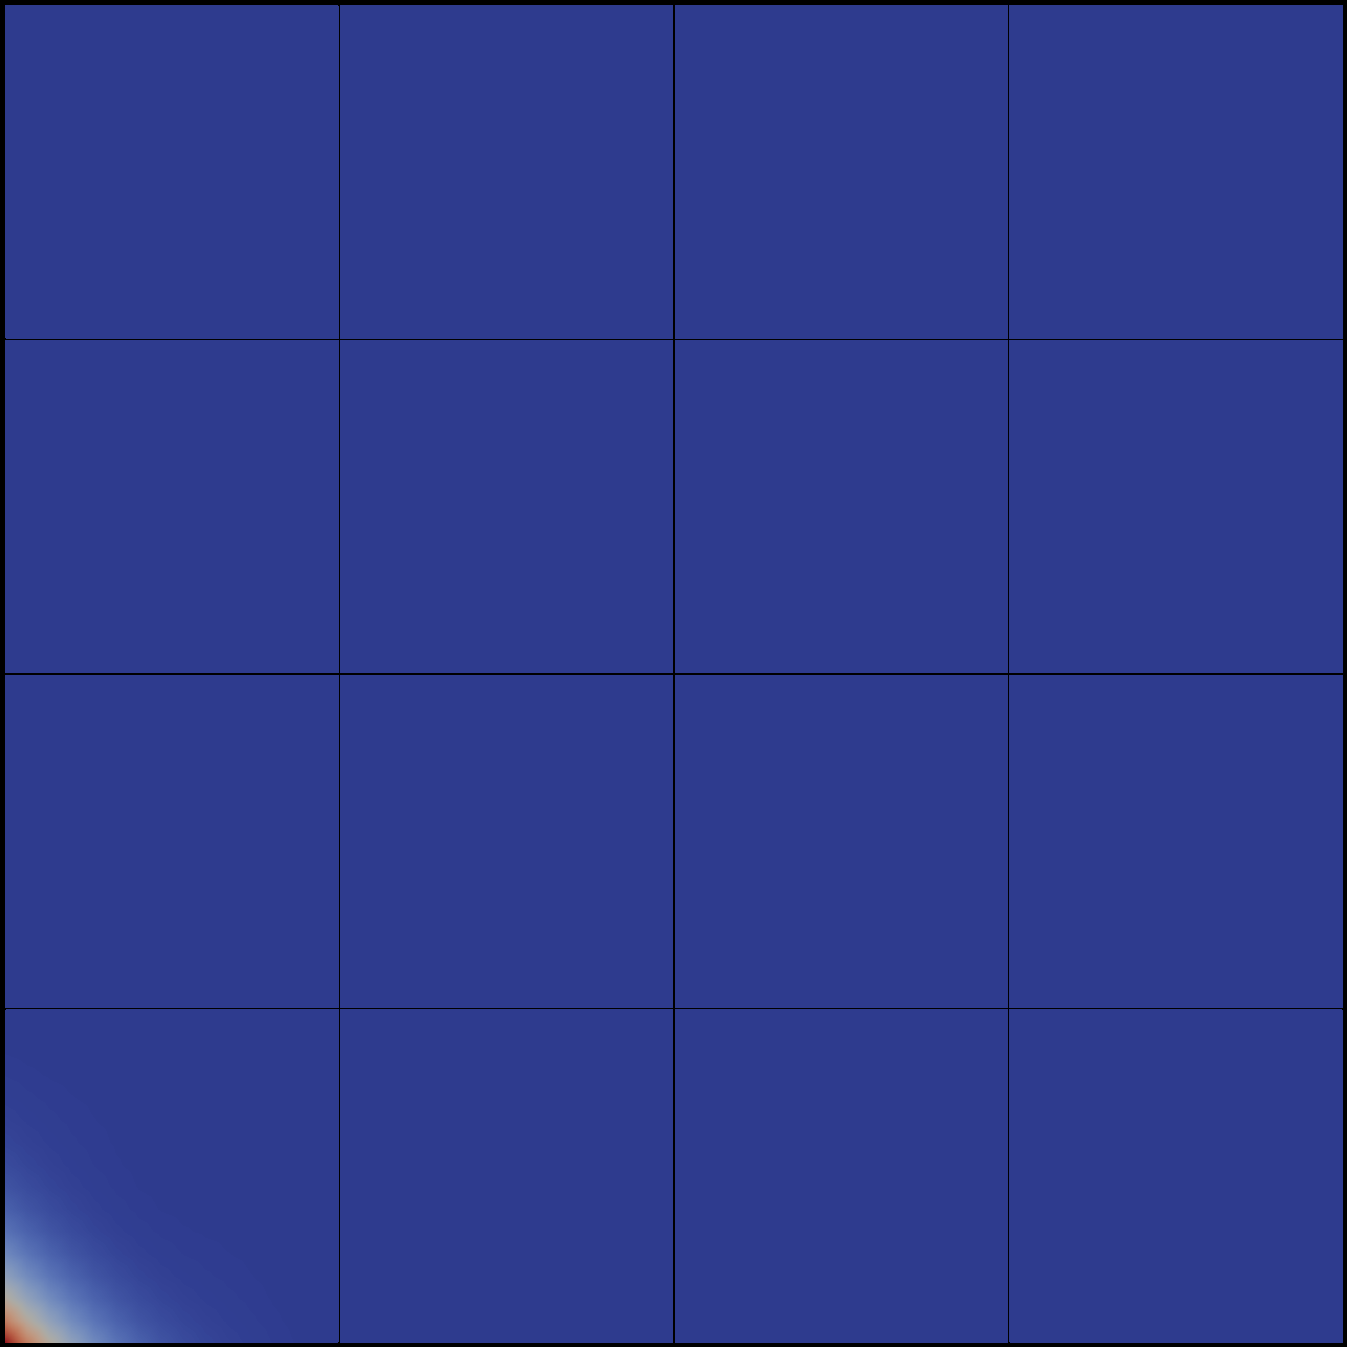
\includegraphics[width=0.45\textwidth]{Chapter_adaptive_mesh_refinement/media/load_imbalance_initial}\label{fig:mesh_imbalance_initial}}
	\hfill
	\subfloat[Mesh after refining]
	{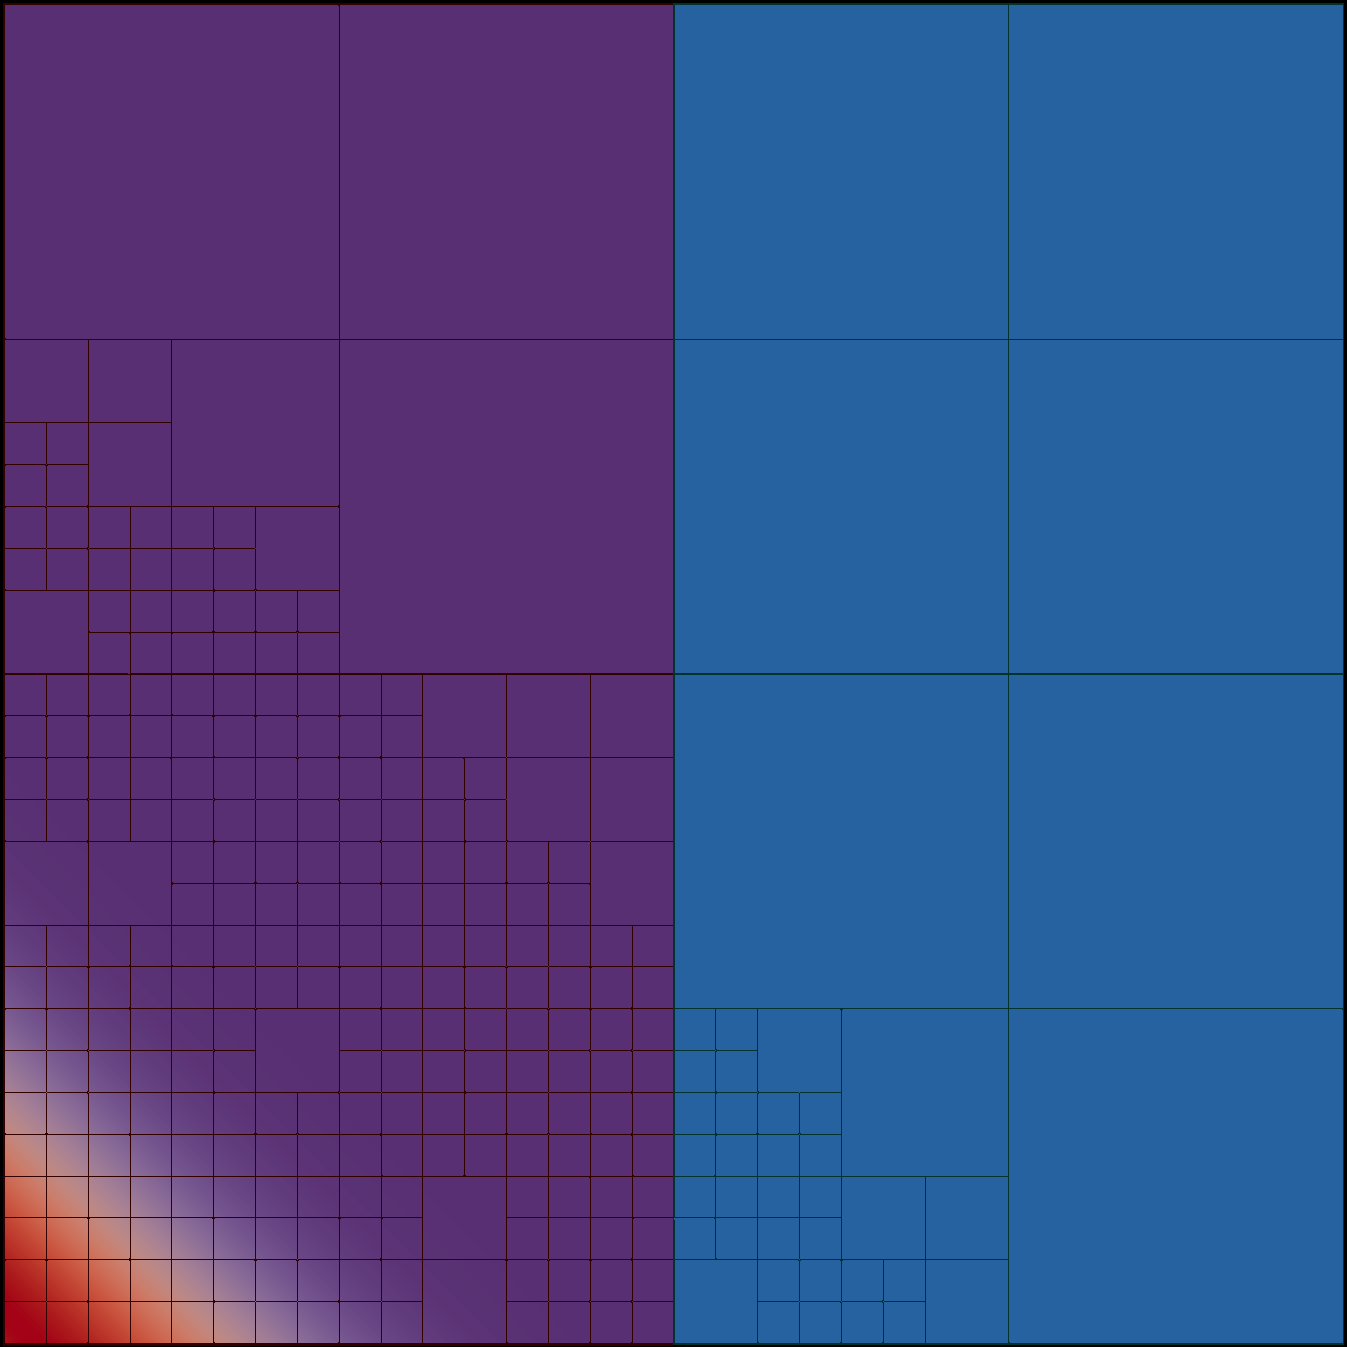
\includegraphics[width=0.45\textwidth]{Chapter_adaptive_mesh_refinement/media/load_imbalance}\label{fig:mesh_imbalance_after_refinement}}
	\caption{Load imbalance: The elements have split unequally in the two worker \acrshortpl{acr:GPU}, denoted in purple and blue, one having a higher computational load. (a) Before refining (b) After refining}\label{fig:load_imbalance}
\end{figure}

The implication of \acrshort{acr:AMR} in the context of high performance computing, the central
challenge of this thesis, is the appearance of load imbalance and loss of computing efficiency on
and between processors. For example, the mesh from Figure~\ref{fig:mesh_refinement} is split into
two blocks for two \acrshortpl{acr:GPU} to work in parallel, as shown on
Figure~\ref{fig:load_imbalance}. Initially, both the left (purple) and right (blue)
\acrshortpl{acr:GPU} have the same number of elements in their domain. After refining, the left
\acrshort{acr:GPU} has more elements as the wave is in its domain and more elements have split
there. Elements will have to be sent from the left \acrshort{acr:GPU} to the right
\acrshort{acr:GPU} in order to even out the computational load, while ensuring that there are as few
interfaces as possible between the \acrshortpl{acr:GPU}. Interfaces need to be minimised because the
\acrshortpl{acr:GPU} need to communicate at every timestep when computing fluxes on these
interfaces. This involves transfers from the \acrshortpl{acr:GPU} to their \acrshort{acr:CPU},
between \acrshortpl{acr:CPU}, and finally back from the \acrshortpl{acr:CPU} to their
\acrshort{acr:GPU}. This happens twice, once for each side of the interface. This is an expensive
process, and improving locality of the elements will help reduce the runtime of that part of the
computation. This is known as dynamic load balancing, and Chapter~\ref{chapter:load_balancing} is
dedicated to solving this problem.

\section{Error Estimation}\label{section:adaptive_mesh_refinement:error_estimation}

We cannot simply refine everywhere in the domain at every occasion, since this is no better than
having a finer mesh to start with. The mesh must only be refined where the expected error is higher.
We therefore estimate the error of each element of the mesh, then refine only those elements which
require better resolution.

As noted in Chapter~\ref{chapter:spectral_element_method}, we represent the solution as an infinite
series of polynomials. In this case we use the Legendre polynomials \(L_n(x)\) of degree \(n\), with
the coefficients \(a_n\) being the modes of the solution.

\begin{equation} \label{equ:infinite_sum_amr}
	u(x) = \sum_{n = 0}^{\infty}a_n L_n(x)
\end{equation}

It is of course impossible to use an infinite sum on computers, therefore we truncate this sum to
\(N\), the polynomial order of the solution. The remaining terms, denoted by \(\tau \), are the
truncation error of the solution.

\begin{equation} \label{equ:solution_approximation}
	\begin{aligned}
		u(x) &= \sum_{n = 0}^{\infty } a_n L_n(x) \\
		&= \sum_{n = 0}^{N}a_n L_n(x) + \sum_{n = N + 1}^{\infty }a_n L_n(x) \\ 
		&= \sum_{n = 0}^{N}a_n L_n(x) + \tau \\
		&\approx \sum_{n = 0}^{N}a_n L_n(x)
	\end{aligned}
\end{equation}

The norm of the truncation error provides an estimate of the overall error of the solution. To find
it, we will need the modes \(a_n\) beyond \(N\), which can be obtained by extrapolation of the known
modes \(a_n, n = 0 \cdots N\). The polynomials we use are orthogonal, therefore the following simple
relation holds for the inner product of two of the polynomials.

\begin{equation} \label{equ:polynomial_orthogonality}
	\begin{aligned}
		\left( L_n, L_m \right) &= \int_{-1}^{1}L_n(r)L_m(r)dr \\
		&= \frac{2}{2n + 1}\delta _{n m}
	\end{aligned}
\end{equation}

\noindent
with \(\delta_{n m}\) being the Kronecker delta. We start by computing the known modes by taking the
inner product of the approximate solution \(u_h(x)\) and  the corresponding Legendre polynomial
\(L_n(x)\).

\begin{equation} \label{equ:modes_inner_product}
	\begin{aligned}
		\left( u_h, L_n \right) &= \int_{-1}^{1} u_h(x(r)) L_n(r) dr \\
		&= \sum_{k = 0}^{N} a_k \int_{-1}^{1} L_k(r) L_n(r)dr \\
		&= \frac{2}{2n + 1} a_n
	\end{aligned}
\end{equation}

\noindent
Rearranging, we get the modes \(a_n\).

\begin{equation} \label{equ:modes}
	a_n = \frac{2n + 1}{2}\int_{-1}^{1}u_h(x(r))L_n(r)dr
\end{equation}

\noindent
If we can obtain the truncated modes by extrapolation of our known modes \(a_n\), the \(L_2\) norm
of the truncation error can then be approximated.

\begin{equation} \label{equ:error_norm}
	\begin{aligned}
		\left \| \tau \right \| \approx \tau_{est} &= \sqrt{\int_{-1}^{1} \sum_{n = N + 1}^{\infty } {\left( \widetilde{a}_n L_n(r) \right)}^2 dr} \\
		&= \sqrt{\sum_{n = N + 1}^{\infty }\widetilde{a}_n^2 \int_{-1}^{1} L_n(r) L_n(r) dr},
	\end{aligned}
\end{equation}

\noindent
where \(\widetilde{a}_n\) are the extrapolated modes. We use the orthogonality of the Legendre
polynomials shown in Equation~\ref{equ:polynomial_orthogonality} to obtain a simpler form of the
truncation error norm.

\begin{equation} \label{equ:error_norm_1D}
	\tau_{est} = \sqrt{\sum_{n = N + 1}^{\infty } \frac{\widetilde{a}_{n}^2}{\frac{(2n + 1)}{2}}}
\end{equation}

\noindent
In 2D, the solution is a tensor product of polynomials, so the truncation error changes accordingly. 

\begin{equation} \label{equ:error_norm_2D}
	\tau_{est} = \sqrt{\sum_{n = N + 1}^{\infty } \sum_{m = M + 1}^{\infty}\frac{\widetilde{a}_{nm}^2}{\frac{(2n + 1)(2m + 1)}{2^2}}}
\end{equation}

Furthermore, the decay rate of the modes provides an indication of the quality of the solution, in
addition to a model for error estimation. For a smooth function, in this context this means a
well-resolved solution, the modes \(a_n\) decay exponentially. As per~\cite{Mavriplis1990}, we model
the exponential decay as follows

\begin{equation} \label{equ:exponential_decay}
	a_n = Ce^{-\sigma n}
\end{equation}

\noindent
by least squares best fit to the existing calculated modes \(a_n, n = 0 \cdots N\).
Figure~\ref{fig:sin_read_modes} shows an example with the modes of the smooth function \(u = \sin(\pi
x)\) with a polynomial order \(N = 15\). It can be observed that the decay of the modes start
slowly, but decays exponentially after the first few modes. Figure~\ref{fig:sin_computed_modes}
shows the modeled \(a_n\), with the dotted line being the slope \( \sigma \).

\begin{figure}[H]
	\centering
	\subfloat[Modes of the solution]
	{\includesvg[width=0.45\textwidth]{Chapter_adaptive_mesh_refinement/media/modes_N15}\label{fig:sin_read_modes}}
	\hfill
	\subfloat[Modeled modes]
	{\includesvg[width=0.45\textwidth]{Chapter_adaptive_mesh_refinement/media/modes_computed_N15}\label{fig:sin_computed_modes}}
	\caption{Modes of the solution: We use the known modes and their decay rate to eventually
	extrapolate unknown modes. (a) Known modes (b) Modeled exponentially decaying modes}\label{fig:sin_modes}
\end{figure}

In order to fit a straight line to the data by linear least-squares, we want a linear relation
between the decay rate \(\sigma \) and the modes. We take the logarithm of both sides of
Equation~\ref{equ:exponential_decay} and get our linear relation.

\begin{equation} \label{equ:exponential_decay_linear}
	\ln(a_n) = \ln(C) - \sigma n
\end{equation}

\noindent
We apply a linear least-squares fit to the last points of the known modes \(a_n\). The slope of the
line, \(\sigma \), is the error refinement criterion. It will help choose a refinement strategy in
Section~\ref{section:adaptive_mesh_refinement:refinement_criteria}. The linear least-squares fit
finds a straight line by minimising the sum of the squares of the distances between the fitted
points and the line. The resulting line is given by:

\begin{equation}
	y = \alpha + \beta x,
\end{equation}

\noindent
and its coefficients are computed by:

\begin{align}
	& \beta = \frac{\sum_{i = 1}^{n}(x_i - \overline{x})(y_i - \overline{y})}{\sum_{i = 1}^{n}{(x_i -\overline{x})}^2}, \\
	& \alpha = \overline{y} - \beta \overline{x},
\end{align}

\noindent
with \(\overline{x}\) and \(\overline{y}\) being the averages of the \(x\) and \(y\) data
respectively. The \(x\) data is the mode number \(n = 0 \cdots N\), and the \(y\) data are the known
modes in log form, \( \log(a_n) \).The error decay slope becomes \(\sigma = - \beta \), and the constant becomes \(C =
e^\alpha \).

Back to the error estimation, we can replace the sums of~\ref{equ:error_norm_1D}
and~\ref{equ:error_norm_2D} by integrals since the behaviour of the modes is known as an analytic
function of \(n\).

\begin{align}
	&1D: \quad \tau_{est} = \sqrt{\sum_{n = N + 1}^{\infty } \frac{\widetilde{a}_n^2}{\frac{2n + 1}{2}}} 
			   \Rightarrow \sqrt{\int_{N + 1}^{\infty } a_n^2 dn}, \label{equ:error_1D}
	\\
	&2D: \quad \tau_{est} = \sqrt{\sum_{n = N + 1}^{\infty }\sum_{m = M + 1}^{\infty}\frac{\widetilde{a}^2_{nm}}{\frac{(2n + 1)(2m + 1)}{2^2}}}
			   \Rightarrow \sqrt{\int_{M+1}^{\infty }\int_{N + 1 }^{\infty}{(a_{nm})}^2 dn dm} \label{equ:error_2D}
\end{align}

\noindent
By using the exponential decay model of Equation~\ref{equ:exponential_decay}, the 1D case can be
evaluated directly.

\begin{equation}
	\begin{aligned}
		\tau_{est} &= \sqrt{\int_{N + 1}^{\infty } a_n^2 dn} \\
		&= \sqrt{\int_{N + 1}^{\infty } {\left( Ce^{-\sigma n} \right)}^2 dn} \\
		&= \sqrt{\frac{C^2}{2\sigma }}e^{-\sigma (N + 1)}. 
	\end{aligned}
\end{equation}

The same method cannot be applied to the 2D case, as the modes in Equation~\ref{equ:error_2D} are
defined in two dimensions. We will need to fit these modes in 1D to find the error estimate as in
the 1D case. We use the same polynomial order in both \(x\) and \(y\) directions, and create 1D
equivalent modes \(\overline{a}_n\). 

\begin{equation}
	\overline{a}_n = \left| a_{n,n} \right| + \sum_{i = 0}^{n-1} \left( \left| a_{i, n} \right| + \left| a_{n, i} \right| \right)
\end{equation}

\noindent
We use the equivalent modes to estimate the error.

\begin{equation}
	\begin{aligned}
		\tau_{est} &= \sqrt{\int_{M+1}^{\infty }\int_{N + 1 }^{\infty}{(a_{nm})}^2 dn dm} \\
		&= \sqrt{\int_{N + 1}^{\infty }\overline{a}_p^2 dp} \\
		&= \sqrt{\int_{N + 1}^{\infty} Ce^{-2\sigma p}dp} \\
		&= \sqrt{\frac{C}{2\sigma}e^{-2\sigma(N + 1)}} \\
		&= \sqrt{\frac{C}{2\sigma}} e^{-\sigma (N + 1)}
	\end{aligned}
\end{equation}

\noindent
The error estimator constants \(\sigma \) and \(C\) are computed from the 1D equivalent modes
\(\overline{a}_n\).

It is now possible to refine when the estimated error is past a certain threshold. We still need to
choose one of the refinement strategies from
Section~\ref{section:adaptive_mesh_refinement:refinement_strategies}.
Section~\ref{section:adaptive_mesh_refinement:refinement_criteria} describes a method to choose the
most appropriate strategy using the error decay rate \(\sigma \) computed previously.

\section{Refinement Criteria}\label{section:adaptive_mesh_refinement:refinement_criteria}

Once we compute the error estimate on every element and know which elements we want to refine, we
must choose how to refine them. Recall from
Section~\ref{section:adaptive_mesh_refinement:refinement_strategies} that we can choose
p-refinement, increasing the polynomial order \(N\) of an element, or h-refinement, splitting the
element into smaller elements to increase the total number of elements \(K\).

The method~\cite{Mavriplis1990} used here is to look at the decay rate of the modes \(a_n\) of the
solution. The error decay rate \(\sigma \) computed in
Section~\ref{section:adaptive_mesh_refinement:error_estimation} is the negative slope of the last
few modes of the solution. A well-resolved solution should have a fast decay of the modes, with
\(\sigma > 1\). On the other hand, \(\sigma \leqslant 1\) implies the solution is not well resolved
as is. Figure~\ref{fig:decaying_modes} compares a poorly resolved solution whose modes do not decay
fast to a well resolved solution whose modes decay fast.

\begin{figure}[H]
	\centering
	\subfloat[Poorly resolved solution]
	{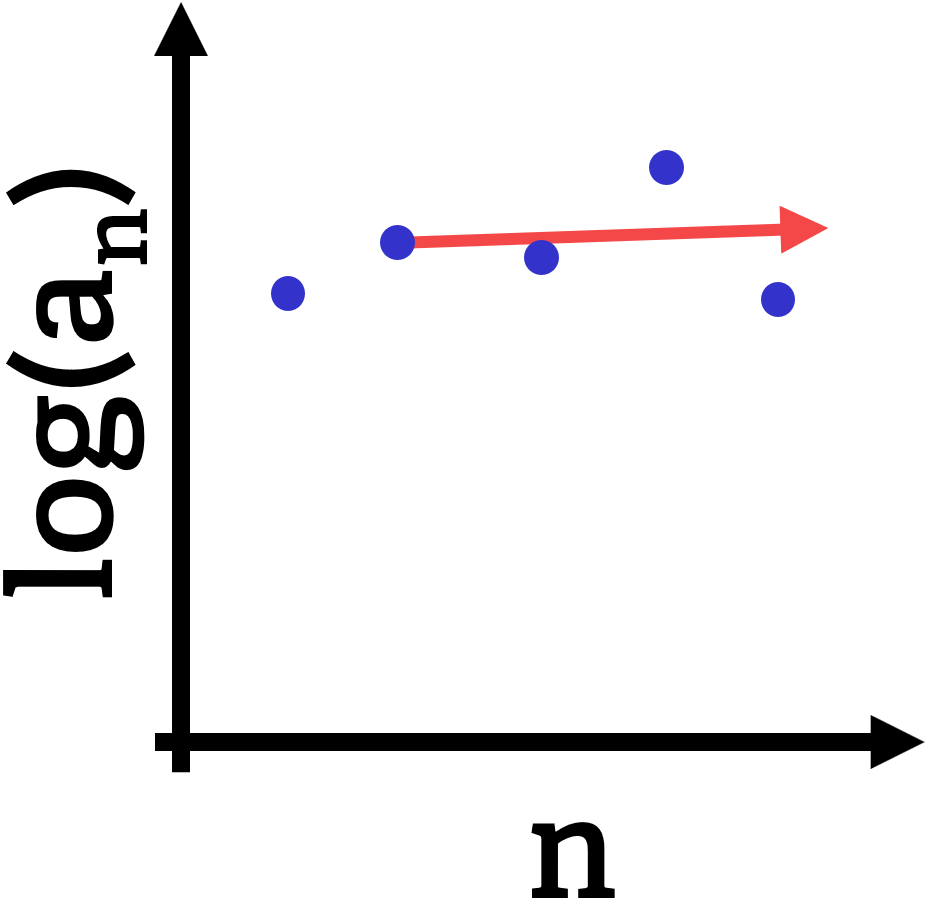
\includegraphics[width=0.4\textwidth]{Chapter_adaptive_mesh_refinement/media/decaying_modes_slow}\label{fig:decaying_modes_slow}}
	\hfill
	\subfloat[Well resolved solution]
	{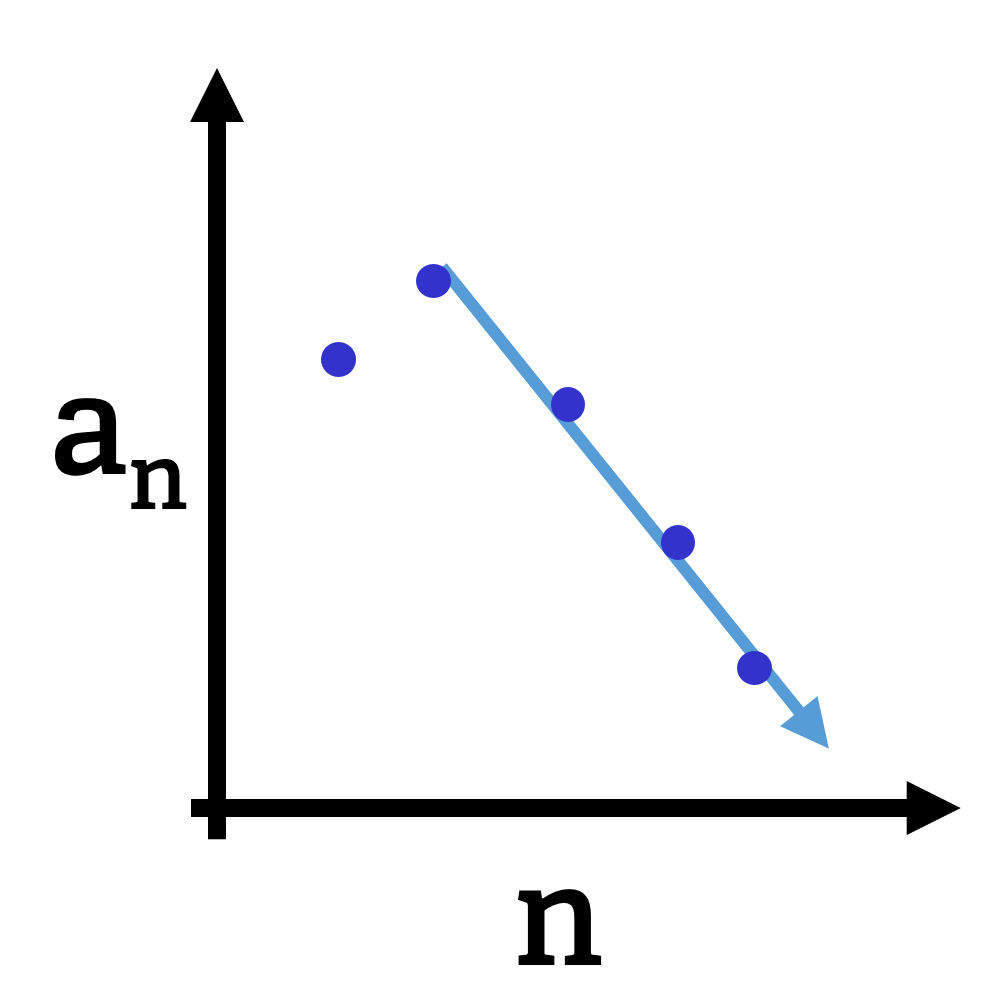
\includegraphics[width=0.4\textwidth]{Chapter_adaptive_mesh_refinement/media/decaying_modes_fast}\label{fig:decaying_modes_fast}}
	\caption{Modes decaying: Decay of spectral modes within an element and their best fit line. (a) \(\sigma \leqslant 1\) (b) \(\sigma > 1\)}\label{fig:decaying_modes}
\end{figure}

The truncation error is related to the value of the extrapolated modes. If the slope of the modes is
steep, each added mode is expected to reduce the error significantly. This is because the truncated
modes have successively much smaller values, therefore the truncated part of the solution is also
small. On the other hand, a flat slope indicates that the value of the modes does not decay fast,
and adding additional modes is not expected to reduce the truncation error much. This is often the
case in non-smooth parts of the solution.

We choose the slope of the modes, \(\sigma \), as our error refinement criterion. If \(\sigma > 1\),
adding polynomial modes is expected to reduce the error significantly, so we use p-refinement and
increase the polynomial order \(N\) of the element. If \(\sigma \leqslant 1\), adding more modes is
not predicted to reduce the error by much, therefore we use h-refinement and split the element into
smaller elements, increasing \(K\).

\section{The Mortar Element Method}\label{section:adaptive_mesh_refinement:mortar_element_method}

One issue that can arise from \acrshort{acr:AMR} is the presence of non-conforming interfaces. The
flux calculations from Chapter~\ref{chapter:spectral_element_method} involve taking the extrapolated
values of the solution of two elements at their interface, and computing the flux at points along
the interface from the two adjacent elements. The elements can then use these fluxes to compute
their derivative for that row or column. This works well when the interfaces are conforming, because
the extrapolated solution values, at the intersection of the thin and bold black lines on
Figure~\ref{fig:conforming_interfaces}, line up between elements.

\begin{figure}[H]
	\centering
	\includesvg[width=0.6\textwidth]{Chapter_adaptive_mesh_refinement/media/conforming_interface_N4}
	\caption{Conforming elemental interface: The extrapolated solution lines up between elements.}\label{fig:conforming_interfaces}
\end{figure}

Once the mesh has been refined, the extrapolated values may not line up anymore, as seen in
Figure~\ref{fig:non_conforming_interfaces}. This makes it impossible to compute fluxes directly, as
the flux computations need a left and right value at every point. These are non-conforming
interfaces. There are three types of non-conforming interfaces. Geometrically non-conforming
interfaces appear when two elements of the same polynomial order do not line up, either because they
are not the same size or because they are offset. Functionally non-conforming interfaces appear when
two elements line up but have a different polynomial orders. Finally, an interface can be both
geometrically and functionally non-conforming.

\begin{figure}[H]
	\centering
	\includesvg[width=0.6\textwidth]{Chapter_adaptive_mesh_refinement/media/non_conforming_interfaces_N4_N6}
	\caption{Non-conforming elemental interfaces: The extrapolated solution does not line up between elements.}\label{fig:non_conforming_interfaces}
\end{figure}

We could simply interpolate values on the points that do not line up, but we want to conserve the
fast convergence of the higher-order methods. We therefore use the mortar element method
from~\cite{Maday1989}. This method adds mortar, or faces, between the elements. These faces have
their own collocation points, unto which the extrapolated solution from the elements is projected.
The flux computations can then be performed on the face's collocation points and be projected back
to the elements afterwards.

\begin{figure}[H]
	\centering
	\includesvg[width=0.8\textwidth]{Chapter_adaptive_mesh_refinement/media/mortar_element_method_N4_N6}
	\caption{The mortar element method: Mortar is added between the elements, shown in blue.}\label{fig:mortar_element_method}
\end{figure}

We define the faces as the smallest of the element sides of a connection. This ensures each face
only has one element on either side, their \textit{left} and \textit{right} elements. Elements can
therefore have multiple faces on each of their sides. The functional of the face has the polynomial
order of the highest-order of its neighbours. The next sections describe how to project to and from
these new faces. The flux calculations are performed on the faces as described in
Section~\ref{chapter:spectral_element_method}. 

\subsection{Projection from Element to Mortar}\label{subsection:adaptive_mesh_refinement:mortar_element_method:element_to_mortar}

\begin{figure}[H]
	\centering
	\includesvg[width=0.6\textwidth]{Chapter_adaptive_mesh_refinement/media/element_to_mortar_N4_N6}
	\caption{Element to mortar projection: The elements' boundary values are projected to the face.}\label{fig:element_to_mortar}
\end{figure}

Elements are denoted \(\Omega \) and faces are denoted \(\Xi \). We will use two coordinates, \(s\)
for the element side coordinate and \(z\) for the face side coordinate. We project to the faces,
therefore the face space will be used as a reference, \(z \in [-1, 1]\). The coordinate change from
element to face has the form \(s = a + bz\), where \(a\) and \(b\) are scalars computed for each
face side when generating the mesh. We can then define the element boundary solution \(U\) and its
projection on the face \(\Psi \). 

\begin{align} 
	& U(s) = \sum_{k = 0}^{N} U(s_k) l_k(s), \label{equ:element_boundary_solution} \\
	& \Psi (z) = \sum_{k = 0}^{J} \Psi(z_k) l_k(z) \label{equ:face_projected_solution}
\end{align}

\noindent
with \(l\) being the Lagrange polynomials, \(N\) being the element polynomial order, and \(J\) being
the face polynomial order. We then require that the integral of the error between the solution and
its projection weighted by the Lagrange polynomials be zero. 

\begin{equation} \label{equ:zero_error}
	\int_{-1}^{1} \left( \Psi (z) - U(a + bz) \right) l_j^\Xi dz = 0, \quad j = 0, \ldots,J
\end{equation}

Incorporating Equation (\ref{equ:element_boundary_solution}) and (\ref{equ:face_projected_solution}),
we get a relation for the boundary and projected solutions.

\begin{equation} \label{equ:boundarry_and_projected}
	\int_{-1}^{1} \sum_{m = 0}^{J} \Psi (z_m) l_m^\Xi (z) l_j ^ \Xi(z) dz = \\
	\int_{-1}^{1} \sum_{k = 0}^{N} U(a + b z_k) l_k^\Omega (a + b z) l_j ^ \Xi (z) dz, \\ \quad
	j = 0, \ldots, J
\end{equation}

Or, in matrix form:

\begin{equation}
	M \Psi = S U
\end{equation}

We can isolate the projected solution.

\begin{equation}
	\Psi = M^{-1} S U
\end{equation}

We use \textit{Gaussian quadrature} to evaluate \(M\) and \(S\). The orthogonality of the Legendre
polynomials will be used to simplify the matrices.

\begin{equation} \label{equ:orthogonality_M}
	l_m (z_k) l_j (z_k) = \\
	\delta _{mk} \delta _{j k} = \left \{ \begin{matrix*}[l]
	& 1, & if & m = k = j \\ 
	& 0, & if & m \neq k \; or \; j \neq k
	\end{matrix*}\right.
\end{equation}

\begin{equation} \label{equ:matrix_M}
	\begin{aligned}
		M_{jm} &= \int_{-1}^{1} l_m ^ \Xi (z) l_j ^ \Xi (z) dz \\
		&= \sum_{k = 0}^{J} l_m ^ \Xi (z_k) l_j ^ \Xi (z_k)w_k ^ \Xi \\
		&= \sum_{k = 0}^{J} w_k ^ \Xi \delta_{mk}\delta_{jk}, & j, m = 0, \ldots, J
	\end{aligned}
\end{equation}

\noindent
where \(w_k\) are the same Gauss-Legendre weights used in
Chapter~\ref{chapter:spectral_element_method}. We use Equation~(\ref{equ:orthogonality_M}) to
simplify the matrix \(M\) to a diagonal matrix.

\begin{equation}
	M_{jm} = \left \{ \begin{matrix}
	w_j^{\Xi }, &  m = j \\ 
	0, & m \neq  j
	\end{matrix}\right.
\end{equation}

\noindent
The same can be done for \(S\), with the following orthogonality relation:

\begin{equation} \label{equ:orthogonality_S}
	l_j ^ \Xi (z_m) = \delta_{jm} = \left \{ \begin{matrix*}[l]
	& 1, & if & m = j\\ 
	& 0, & if & m \neq j
	\end{matrix*}\right.
\end{equation}

\begin{equation} \label{equ:matrix_S}
	\begin{aligned}
		S_{jk} &= \int_{-1}^{1} l_k ^ \Omega \left( a + b z \right) l_j ^ \Xi \left( z \right) dz \\
		&= \sum_{m = 0}^{J} l_k ^ \Omega \left( a + b z_m \right) l_j ^ \Xi \left( z_m \right) w_m ^ \Xi \\
		&= \sum_{m = 0}^{J} l_k ^ \Omega \left( a + b z_m \right) w_m ^{\Xi} \delta_{jm}, \quad j = 0, \ldots, J, \: k = 0, \ldots, N.
	\end{aligned}
\end{equation}

\noindent
We use Equation~(\ref{equ:orthogonality_S}) to simplify the matrix \(S\).

\begin{equation}
	S_{jk} = l_k^{\Omega } \left( a + bz_j \right) w_j^{\Xi}, \quad j = 0, \ldots, J, \: k = 0, \ldots, N.
\end{equation}

With \(M\) and \(S\), we can define a projection matrix from element boundary space to face space.

\begin{equation}
	\begin{aligned}
		P_{jk} ^ {\Omega \rightarrow \Xi} &= M^{-1}S \\
		&= {\left( w_j ^{-1} \right)}^{\Xi }  l_k ^ \Omega \left( a + b z_j \right) {\left( w_j \right)}^{\Xi} \\
		&= l_k ^ \Omega \left(a + b z_j \right), \quad j = 0, \ldots, J, \: k = 0, \ldots, N.
	\end{aligned}
\end{equation}

The projection operation from element to faces is therefore:

\begin{align}  \label{projection_element_to_face}
	\Psi &= P_{jk}^{\Omega \rightarrow \Xi} U_k  \\
	&= \sum_{k = 0}^{N}l_k ^ \Omega(a+ b z_j) U(a + b z_k), \quad j = 0, \ldots, J.
\end{align}

\subsection{Projection from Mortar to Element}\label{subsection:adaptive_mesh_refinement:mortar_element_method:mortar_to_element}

\begin{figure}[H]
	\centering
	\includesvg[width=0.6\textwidth]{Chapter_adaptive_mesh_refinement/media/mortar_to_element_N4_N6}
	\caption{Mortar to Element projection: The faces' values are projected to the elements.}\label{fig:mortar_to_element}
\end{figure}

After projecting the element boundary solution to the faces, the fluxes can be computed on the
faces. The result then needs to be projected back to the element boundaries to be useful in
subsequent calculations. The projection from faces to elements is slightly more complicated than the
other way around because we defined faces to have the size of the smallest elements they connect to.
This means that while each face can only have one element on either side, elements can have multiple
faces on each of their sides. The flux solution must then be projected from multiple faces onto each
element edge.

This time, we take the element coordinates as a basis, \(s \in [-1, 1]\). The coordinate change is
the inverse of that of the element to face projection, \(z = \frac{s - a}{b}\). Here \(\Phi \) is
the computed flux on the face, and \(F\) is the projection on the element side. As in the last
subsection, we require that the integral of the error between the flux solution and its projection
multiplied by the test function, the Lagrange polynomials here, be zero.

\begin{equation} \label{equ:zero_error_to_element}
	\int_{-1}^{o'} \left( F(s) - \Phi (\frac{s - a}{b}) \right) l_j^\Omega(s)ds + \\
	\int_{o'}^{1} \left( F(s) - \Phi (\frac{s - a}{b}) \right) l_j^\Omega (s)ds = 0, \\
	\quad j = 0 \ldots N,
\end{equation}

\noindent
This looks very much like the condition we imposed for the element to face projection, except that
the coordinate change is reversed and there are as many integrals as there are faces connecting to
the element edge. In this case there are two, but there could be an arbitrary number. We can get the
projection solution \(F\) out of each face's integral to form an integral over the whole element
edge.

\begin{equation} \label{equ:zero_error_to_element_rewritten}
	\int_{-1}^{1}F(s)l_j^\Omega(s)ds = \\
	\int_{-1}^{o'} \Phi (\frac{s -a}{b}) l_j^\Omega(s)ds + 
	\int_{o'}^{1} \Phi(\frac{s-a}{b})l_j^\Omega(s)ds.
\end{equation}

\noindent
We then rewrite the solutions in Lagrange form.

\begin{gather}
	F(s) = \sum_{m = 0}^{N}F(s_m)l_m^\Omega(s), \\
	\Phi(\frac{s -a}{b}) = \sum_{m = 0}^{J}\Phi(\frac{s_m -a}{b})l_m^\Xi(\frac{s -a}{b}).
\end{gather}

\noindent
Incorporating those in Equation~(\ref{equ:zero_error_to_element_rewritten}):

\begin{equation} 
	\begin{aligned}
		\int_{-1}^{1}F(s_m)l_m^\Omega(s) l_j^\Omega(s)ds &= \int_{-1}^{o'} \Phi(\frac{s_m -a}{b})l_m^\Xi(\frac{s -a}{b}) l_j^\Omega(s)ds \\
		&+ \int_{o'}^{1} \Phi(\frac{s_m -a}{b})l_m^\Xi(\frac{s -a}{b}) l_j^\Omega(s)ds
	\end{aligned}
\end{equation}

\noindent
Or in matrix form:

\begin{equation} 
	MF = S \Phi
\end{equation}

\noindent
We can again isolate the projected solution.

\begin{equation} 
	F = M^{-1} S \Phi
\end{equation}

\noindent
The \(M\) matrix is the same as for the element to face projection.

\begin{equation} \label{equ:matrix_M_face_to_element}
	\begin{aligned}
		M_{jm} &= \int_{-1}^{1}l_m^{\Omega}(s)l_j^{\Omega}(s)ds \\
		&= \sum_{k = 0}^{N} w_k ^{\Omega} \delta_{mk}\delta_{jk}, & j, m = 0, \ldots, J \\
		&= \left \{ \begin{matrix}
			w_j^{\Omega }, & j = m \\ 
			0 & j \neq m.
			\end{matrix}\right.
	\end{aligned}
\end{equation}

\noindent
The \(S\) matrix needs a change of referential from element space \(s\) to face space \(z\) to have
it integrate on faces.

\begin{equation}
	\int_{-1}^{o'} \Phi(\frac{s_m -a}{b})l_m^\Xi(\frac{s -a}{b}) l_j^\Omega(s)ds
	= b\int_{-1}^{1}\sum_{m = 0}^{J} \Phi(z_m)l_m^{\Xi}l_j^{\Omega}(a + bz)dz
\end{equation}

\noindent
\(S\) then becomes: 

\begin{equation}
	\begin{aligned}
		S_{jm} &=  b\int_{-1}^{1}l_m^{\Xi}(z)l_j^{\Omega}(a + bz)dz
		= b\sum_{k = 0}^{J}l_m^{\Xi}(z_k)l_j^{\Omega}(a +b z_k)w_k^{\Xi}, \\
		&= b l_j^{\Omega}(a + bz_m)w_m^{\Xi}, \quad j = 0, \ldots, N, \quad m = 0, \ldots, J.
	\end{aligned}
\end{equation}

\noindent
With \(M\) and \(S\), we can finally define a projection matrix from face space to element boundary
space.

\begin{equation}
	\begin{aligned}
		P^{\Xi \rightarrow \Omega}_{jm} &= M^{-1}S \\
		&= {(w_j^{-1})}^{\Omega } \: b \: l_j^{\Omega }(a + bz_m)w_m^{\Xi}\\
		&= b \: l_j^{\Omega}(a + bz_m)\frac{w_m^{\Xi}}{w_j^{\Omega}}, \quad j = 0, \ldots, N, \: m = 0, \ldots J. 
	\end{aligned}
\end{equation} 

\noindent
The projection operation from faces to elements is therefore:

\begin{align} \label{projection_face_to_element}
	F &= P^{\Xi \rightarrow \Omega}_{jm} \Phi_m  \\
	&= \sum_{m = 0}^{N} b \: l_j^{\Omega}(a + bz_m)\frac{w_m^{\Xi}}{w_j^{\Omega}} \Phi (a + b z_j), \quad j = 0, \ldots, J.
\end{align}

\section{Mesh Pre-conditioning}\label{section:adaptive_mesh_refinement:pre_conditioning}

When initial conditions are applied to a coarse mesh, some error is introduced to the problem. This
error does not reduce with refinement, it simply propagates through the domain. To address this
issue, we implement a simple pre-conditioning algorithm. The algorithm advances the solution in
time, refines it, then sets the initial conditions again. This is an iterative process, and can be
performed multiple times. This is what will be called pre-condition steps. The refinement interval
dictates how many time steps are computed before refining and resetting the initial conditions. The
performance of this algorithm is assessed in Section~\ref{section:results:adaptivity_performance}.

\section{Implementation}\label{section:adaptive_mesh_refinement:implementation}

As detailed in Chapter~\ref{chapter:graphics_processing_units}, the grid is stored on the
\acrshort{acr:GPU} as a flat vector of elements, each element having pointers to its solution
arrays, stored in \acrshort{acr:GPU} dynamic memory. This ensures the elements have a fixed size
regardless of their polynomial order. The element vector is allocated in \acrshort{acr:GPU} memory
by the \acrshort{acr:CPU} using the \acrshort{acr:CUDA} runtime. Only this memory can be transferred
between the \acrshort{acr:CPU} and \acrshort{acr:GPU}. Elemental solution arrays cannot be
transferred between the \acrshort{acr:CPU} and \acrshort{acr:GPU} since they are allocated on the
\acrshort{acr:GPU}. The same goes for the faces of the grid. Since the grid is unstructured, the
elements and faces store the index of their neighbours. The faces have one element on either side,
and the elements can have one or multiple faces on each of their four sides.

With that structure in mind, \acrlong{acr:AMR} must be able to add elements to the mesh, change the
polynomial order of elements, replace elements that have split, create, replace and change the
polynomial order of faces, and keep the element and face references coherent. The whole adaptivity
process happens in parallel on each \acrshort{acr:GPU}, each on its mesh block. The adaptivity
process starts by calculating the error in parallel on each element on the \acrshort{acr:GPU}. The
elements store their estimated error \(\tau_{est}\) and their error refinement criterion \(\sigma
\).

\subsection{Counting refining elements}\label{subsection:adaptive_mesh_refinement:implementation:counting_refining_elements}

We start by finding out the total number of h-refining elements. A reduction~\cite{Harris2007} is
computed on the \acrshort{acr:GPU} on a per-block basis, as described in
Subsection~\ref{subsection:graphics_processing_units:implementation:reductions}. In this reduction
each thread examines the estimated error \(\tau_{est}\) of an element against a set threshold and
marks it as refining or not. If refining, the error refinement criterion \(\sigma \) is read to mark
it as h or p refining. If h-refining, the thread sets to 1 the value of an intermediate array at the
thread's index within the block. Then, through a sequence of synchronisations and additions, the
threads add up those values until the block total is known. The block total is then written to an
output vector at the block's index within the mesh.

Once this is done, the array with each block's total number of h-refining elements is copied to the
\acrshort{acr:CPU} and the total number of splitting elements is computed by adding all the values.
Although it would be possible to launch this kernel again with fewer blocks on the resulting vector
to reduce further to fewer values, this would not fill the \acrshort{acr:GPU}. Having the sum be
defined with the same blocks as the elements will help us later when we want to know where to place
new elements in the element vector.

If no elements split in the mesh, we can skip the next steps and only p-refine the elements in
place. In this case, a kernel is launched on the \acrshort{acr:GPU} and p-refining elements will
resize their solution arrays and project their solution onto the new array. The faces can then
increase their polynomial order if either of their neighbour elements has increased their polynomial
order beyond that of the face. 

\subsection{Moving elements}\label{subsection:adaptive_mesh_refinement:implementation:moving_elements}

If any element h-refines, it will create more elements and the element vector will need to be
resized. A new vector is created in \acrshort{acr:GPU} memory by the \acrshort{acr:CPU} with the new
increased size. A prefix sum vector is created for each block of threads, indicating how many
elements have split before it. This tells threads where to put existing and new elements in the new
vector. A kernel is launched on the \acrshort{acr:GPU}, and all elements are assigned to threads and
will either move, p-refine or h-refine. Figure~\ref{fig:refinement_offset} shows a mesh with 6
elements refining, with two elements being h-refined in red.

\begin{figure}[H]
	\centering
	\includesvg[height=0.3\textwidth]{Chapter_adaptive_mesh_refinement/media/refinement_offset}
	\caption{Moving elements from the old vector to the new: Two elements are h-refined (in red), the others are moved.}\label{fig:refinement_offset}
\end{figure}

Non-refining elements are simply moved to their new index in the new vector. This is not a very
costly operation because the element structure only contains geometric data, error data and pointers
to solution data. The solution data itself, representing most of the element's size, is stored in
dynamic memory on the \acrshort{acr:GPU}. It does not need to be copied, only the pointer to it
needs to be copied in the new element vector. 

\noindent
p-refining elements act a bit like non-refining elements, except that they need to create new
solution arrays with their new polynomial order and project their solution to it.

\noindent
h-refining elements create four smaller elements in the new vector. They are placed consecutively at
the new index of the splitting element, in an order determined by the \acrfull{acr:SFC} used,
detailed in~\ref{chapter:load_balancing}. The solution of the splitting element is projected onto
the smaller elements. Four associated faces have to be created to connect the smaller elements to
each other, as well as a node in the center. 

Once the elements have been moved, their index has changed. All faces need to correct their
neighbour elements' indices to reflect their new indices. The faces use the same block prefix sum as
the elements to find the new index of their neighbours.

This section is prone to race conditions. The new element indices must be computed in parallel to be
efficient, and cannot loop over all elements to find their offset. This would be very slow, and data
residing in other blocks of threads is not as easily accessible. This is where the prefix sum vector
enters. Each thread will know the offset of its block and only need to add the additional number of
elements splitting before it within its block, which is accessible in block-shared memory. This
ensures no threads read or write the same memory location, and can all move their elements directly
to the correct location concurrently.

\subsection{Moving faces}\label{subsection:adaptive_mesh_refinement:implementation:moving_faces}

Faces are refined similarly to elements. If an element on either side of a face splits while the
face covers the whole element side, the face will split too. This ensures that the face always has
the length of the smallest of the two elements it connects to. 

Unlike elements, faces do not need any specific ordering like described in
Section~\ref{section:load_balancing:hilbert_curve}. This simplifies the refinement process for
faces, as moving faces keep the same index and splitting faces add a face at the end of the vector.
Faces also increase their polynomial order if needed. Figure~\ref{fig:refinement_offset_face} shows
an array of faces being refined, with the splitting faces in red adding faces to the end of the new
array. A prefix sum for each block of threads is also computed for faces to permit them to split in
parallel without race conditions.

The splitting faces become two faces each, one at their initial index and another at the end of the
array. Elements must then check their neighbouring faces for splitting, and update the face indices
as needed.

\begin{figure}[H]
	\centering
	\includesvg[height=0.3\textwidth]{Chapter_adaptive_mesh_refinement/media/refinement_offset_faces}
	\caption{Moving faces from the old vector to the new: Two faces split (in red), the others are moved.}\label{fig:refinement_offset_face}
\end{figure}
